% !TEX encoding = UTF-8 Unicode
% $Header: /cvsroot/latex-beamer/latex-beamer/solutions/conference-talks/conference-ornate-20min.en.tex,v 1.6 2004/10/07 20:53:08 tantau Exp $

\documentclass{beamer}

\mode<presentation>
{
  \usetheme{Warsaw}
  % or ...

  \setbeamercovered{transparent}
  % or whatever (possibly just delete it)
  
  \setbeamertemplate{navigation symbols}{}
  
  \newcommand*\oldmacro{}%
  \let\oldmacro\insertshorttitle%
  \renewcommand*\insertshorttitle{%
    \oldmacro\hfill%
    \insertframenumber\,/\,\inserttotalframenumber}
}

\usepackage[utf8]{inputenc}
% or whatever

\usepackage{times}
\usepackage{multirow}
\usepackage[T1]{fontenc}
\usepackage[french]{babel}
\usepackage{graphicx}

\usepackage{eso-pic}
\usepackage{color}
\usepackage{tikz}
\usepackage{wasysym}

% Or whatever. Note that the encoding and the font should match. If T1
% does not look nice, try deleting the line with the fontenc.

%\title[Petit guide des bonnes pratiques pour la construction et la maintenance d'$\alpha$-extracteurs cosmiques à vacuité]
{}

\titlegraphic{\raisebox{2em}{}}

\author[Prologin]
{
\includegraphics{../prologin2016}}

\date
{}

\begin{document}

\definecolor{vert}{rgb}{0.07 0.54 0.07}


\begin{frame}
        \centering 
\includegraphics[width=0.9\linewidth]{../prologin2016} \\
        \vspace{1.5cm}
	Petit guide des bonnes pratiques pour la construction et la maintenance d'$\alpha$-extracteurs cosmiques à vacuité
\end{frame}

\begin{frame}
	\frametitle{Présentation}
	\begin{itemize}
        \item Jeu de stratégie à 2 joueurs : \textcolor{green}{\textbf{Vert}} et
            \textcolor{pink}{\textbf{Rose}}
        \item Tour par tour
        \item Carte carrée de taille fixe
	\end{itemize}
\end{frame}

\begin{frame}
	\frametitle{Plateau}
	\center{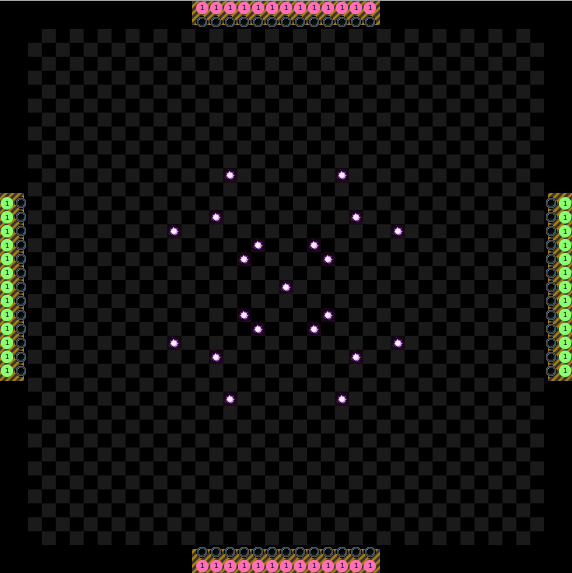
\includegraphics[width=7cm]{pictures/map}}
\end{frame}

\begin{frame}
	\frametitle{Pulsar}
    \begin{columns}[T]
        \begin{column}{.3\textwidth}
            
\includegraphics[width=3cm]{pictures/pulsar}
        \end{column}
        \begin{column}{.7\textwidth}
            \begin{itemize}
                \item Période de pulsation $T$
                \item Puissance d'émission $P$
                \item Nombre de pulsations restantes $R$
            \end{itemize}
        \end{column}
    \end{columns}
\end{frame}

\begin{frame}
	\frametitle{Tuyau}
    \begin{columns}[T]
        \begin{column}{.05\textwidth}
        \end{column}
        \begin{column}{.4\textwidth}
            \center{Simple tuyau} \\
            \vspace{1.5cm}
            
\includegraphics[width=3cm]{pictures/tuyau}
        \end{column}
        \begin{column}{.55\textwidth}
            \center{Super tuyau} \\
            \vspace{0.8cm}
            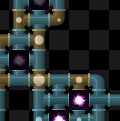
\includegraphics[width=3cm]{pictures/super-tuyau}
        \end{column}
    \end{columns}
\end{frame}

\begin{frame}
	\frametitle{Plasma}
    \begin{columns}[T]
        \begin{column}{.3\textwidth}
            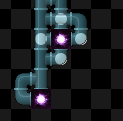
\includegraphics[width=3cm]{pictures/emission}
        \end{column}
        \begin{column}{.7\textwidth}
            \begin{itemize}
                \item Ressource émise par les pulsars
                \item Se déplace dans la direction qui le raproche le plus d'une base
                \item Disparaît s'il n'est relié à aucun tuyau à la fin d'un tour
            \end{itemize}
        \end{column}
    \end{columns}
\end{frame}

\begin{frame}
	\frametitle{Déplacement du plasma}
    \begin{columns}[T]
        \begin{column}{.5\textwidth}
            \center{Se dirige vers la base la plus proche} \\
            \center{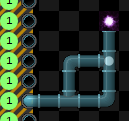
\includegraphics[width=3cm]{pictures/before_division}}
        \end{column}
        \begin{column}{.5\textwidth}
            \center{Se divise en cas d'égalité vers plusieurs directions} \\
            \center{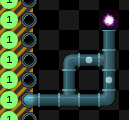
\includegraphics[width=3cm]{pictures/after_division}}
        \end{column}
    \end{columns}
\end{frame}

\begin{frame}
	\frametitle{Base}
    \begin{columns}[T]
        \begin{column}{.3\textwidth}
            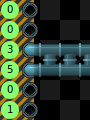
\includegraphics[width=3cm]{pictures/aspiration}
        \end{column}
        \begin{column}{.7\textwidth}
            \begin{itemize}
                \item Case de récolte du plasma
                \item Possède une puissance d'aspiration qui réduit la distance de cette case au reste du plateau
                \item 5 points d'aspirations maximum par case
            \end{itemize}
        \end{column}
    \end{columns}
\end{frame}

\begin{frame}
	\frametitle{Points d'actions}
	\begin{columns}[T]
        \begin{column}{.65\textwidth}
            \begin{itemize}
	            \item[+] commencer un tour
	            \item[\alert{--}] construire un tuyau
	            \item[\alert{--}] améliorer un tuyau
	            \item[\alert{--}] déplacer la puissance d'aspiration
	            \item[\alert{--}] détruire un tuyau/super-tuyau
	            \item[\alert{--}] déblayer un tuyau détruit
	        \end{itemize}
        \end{column}
        \begin{column}{.35\textwidth}
            \begin{itemize}
                \item[] 4
	            \item[] 1
	            \item[] 1
	            \item[] 0 $\rightarrow$ 1
	            \item[] 3/4
	            \item[] 1
            \end{itemize}
        \end{column}
    \end{columns}
\end{frame}

\begin{frame}
    \frametitle{Tournois intermédiaires}
    \begin{itemize}
        \item Samedi 15~h~42 (tournoi test)
        \item Samedi 17~h~42
        \item Samedi 23~h~42
        \item Dimanche 5~h~42
        \item Dimanche 11~h~42
        \item Dimanche 17~h~42
        \item Lundi 00~h~42 (tournoi final)
    \end{itemize}
\end{frame}

\begin{frame}
    \frametitle{Conférences}
    \begin{itemize}
        \item \textbf{Samedi 9~h~50} Benjamin Jean : Open Law
        \item \textbf{Samedi 16~h~00} Jill-Jênn Vie :
        \item \textbf{Samedi 18~h~00} Nicolas Blanchard :
        \item \textbf{Lundi 11~h~45} Xavier Garrigue : Apycat
    \end{itemize}
\end{frame}

\begin{frame}
    \frametitle{Questions}
    Posez vos questions sur le sujet de la finale
\end{frame}

\begin{frame}
    \frametitle{Déroulement}
    TODO ce qu'il va se passer pendant la finale
\end{frame}

\begin{frame}
    \frametitle{Questions}
    Posez vos questions sur le déroulement de la finale
\end{frame}

\end{document}
